\section{Results}\label{sec:results}

\subsection{Model Recovery}\label{sec:recovery}
Fig. \ref{fig:recovery} shows how often BIC selects the generating model, pooled over the three domains (90 data sets per point). In homogeneous populations, the QL generator is identified in 86\%, 93\% and 100\% of data sets with 100, 400 and 1,600 people per order; the Bayes generator in 30\%, 71\% and 98\%; and the anchoring generator in 27\%, 64\% and 97\%. Two errors dominate at small samples. With 100 people per order, data from the Bayes generator are attributed to the QL model in 63 of 90 data sets: with three parameters, the QL model absorbs sampling noise as an apparent order effect. Data from the anchoring generator are attributed to Bayes, because its order effect is small relative to sampling noise. With individual differences, recovery of the QL generator falls to 76\%, 66\% and 79\%, and in the remaining cases Bayes is selected; the average of many slightly different QL people is not itself a QL model. The QQ test rejected the equality for the anchoring generator in 31\%, 39\% and 62\% of data sets (homogeneous) and for the QL generator in at most 4\%, close to the nominal 5\%. The mixture generator was attributed to Bayes in 68--76 of 90 data sets at every sample size.

\begin{figure*}[!t]
\centering
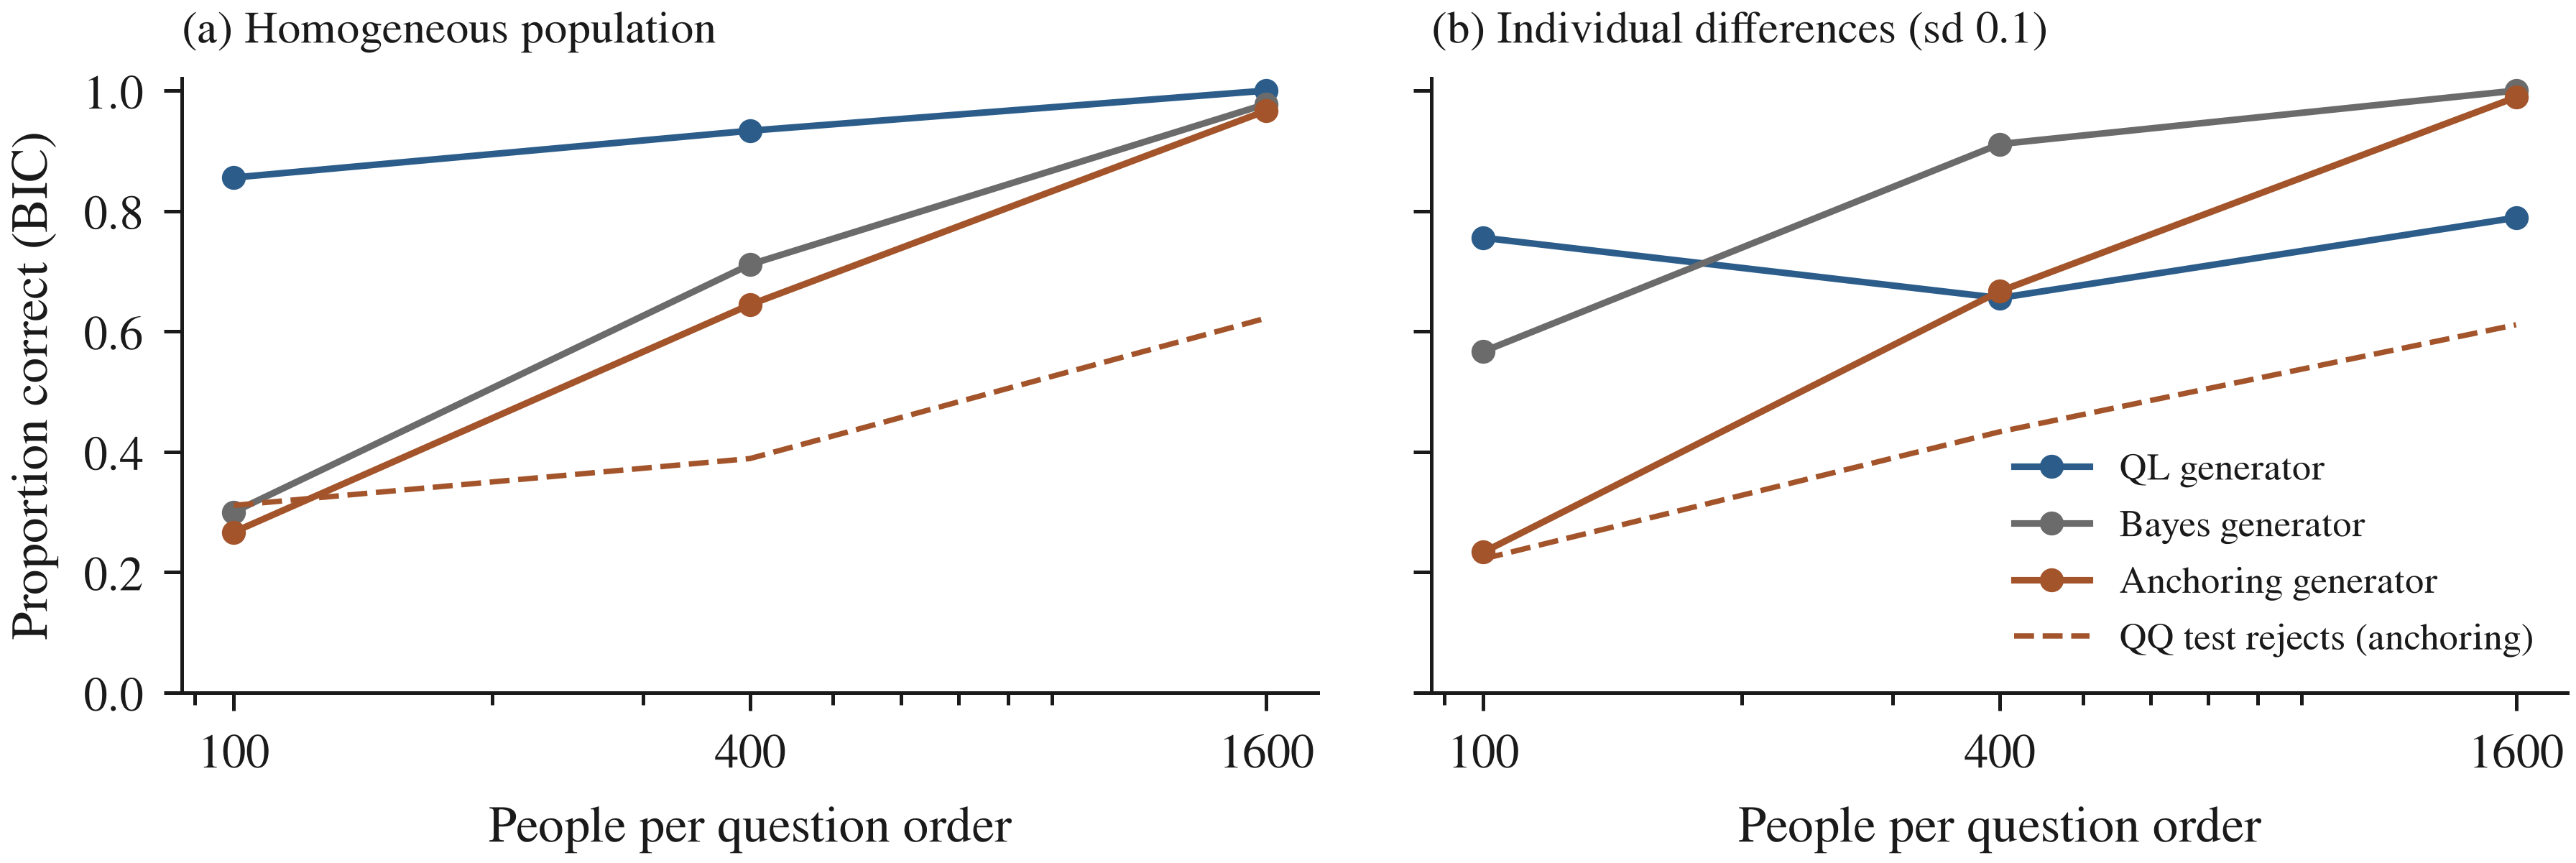
\includegraphics[width=\textwidth]{figures/Fig3_recovery.png}
\caption{Experiment 1: proportion of data sets in which BIC selects the generating model, pooled over three domains (30 repetitions each), against people per question order; dashed line, proportion of anchoring data sets in which the QQ test rejects the equality.}\label{fig:recovery}
\end{figure*}

\subsection{Cross-Order Prediction}\label{sec:crossorder}
Fig. \ref{fig:crossorder} gives the divergence between predicted and true B-first answers. When the generator is QL and the population homogeneous, the QL model predicts best (median KL 0.004 with $N=400$ and 0.0002 with $N=4{,}000$, against 0.014 and 0.011 for Bayes). With individual differences, the advantage shrinks to a tie at $N=400$ (0.013 for both) and a small margin at $N=4{,}000$ (0.007 against 0.010). When the generator is anchoring or the mixture, the QL model is the worst of all models (0.23--0.26 and 0.11--0.13), about ten times worse than Bayes, while Bayes is never worse than 0.03 under any generator. The anchoring models fail badly when the generator is QL or Bayes (0.12--0.19), because their order effect is the wrong shape.

\begin{figure*}[!t]
\centering
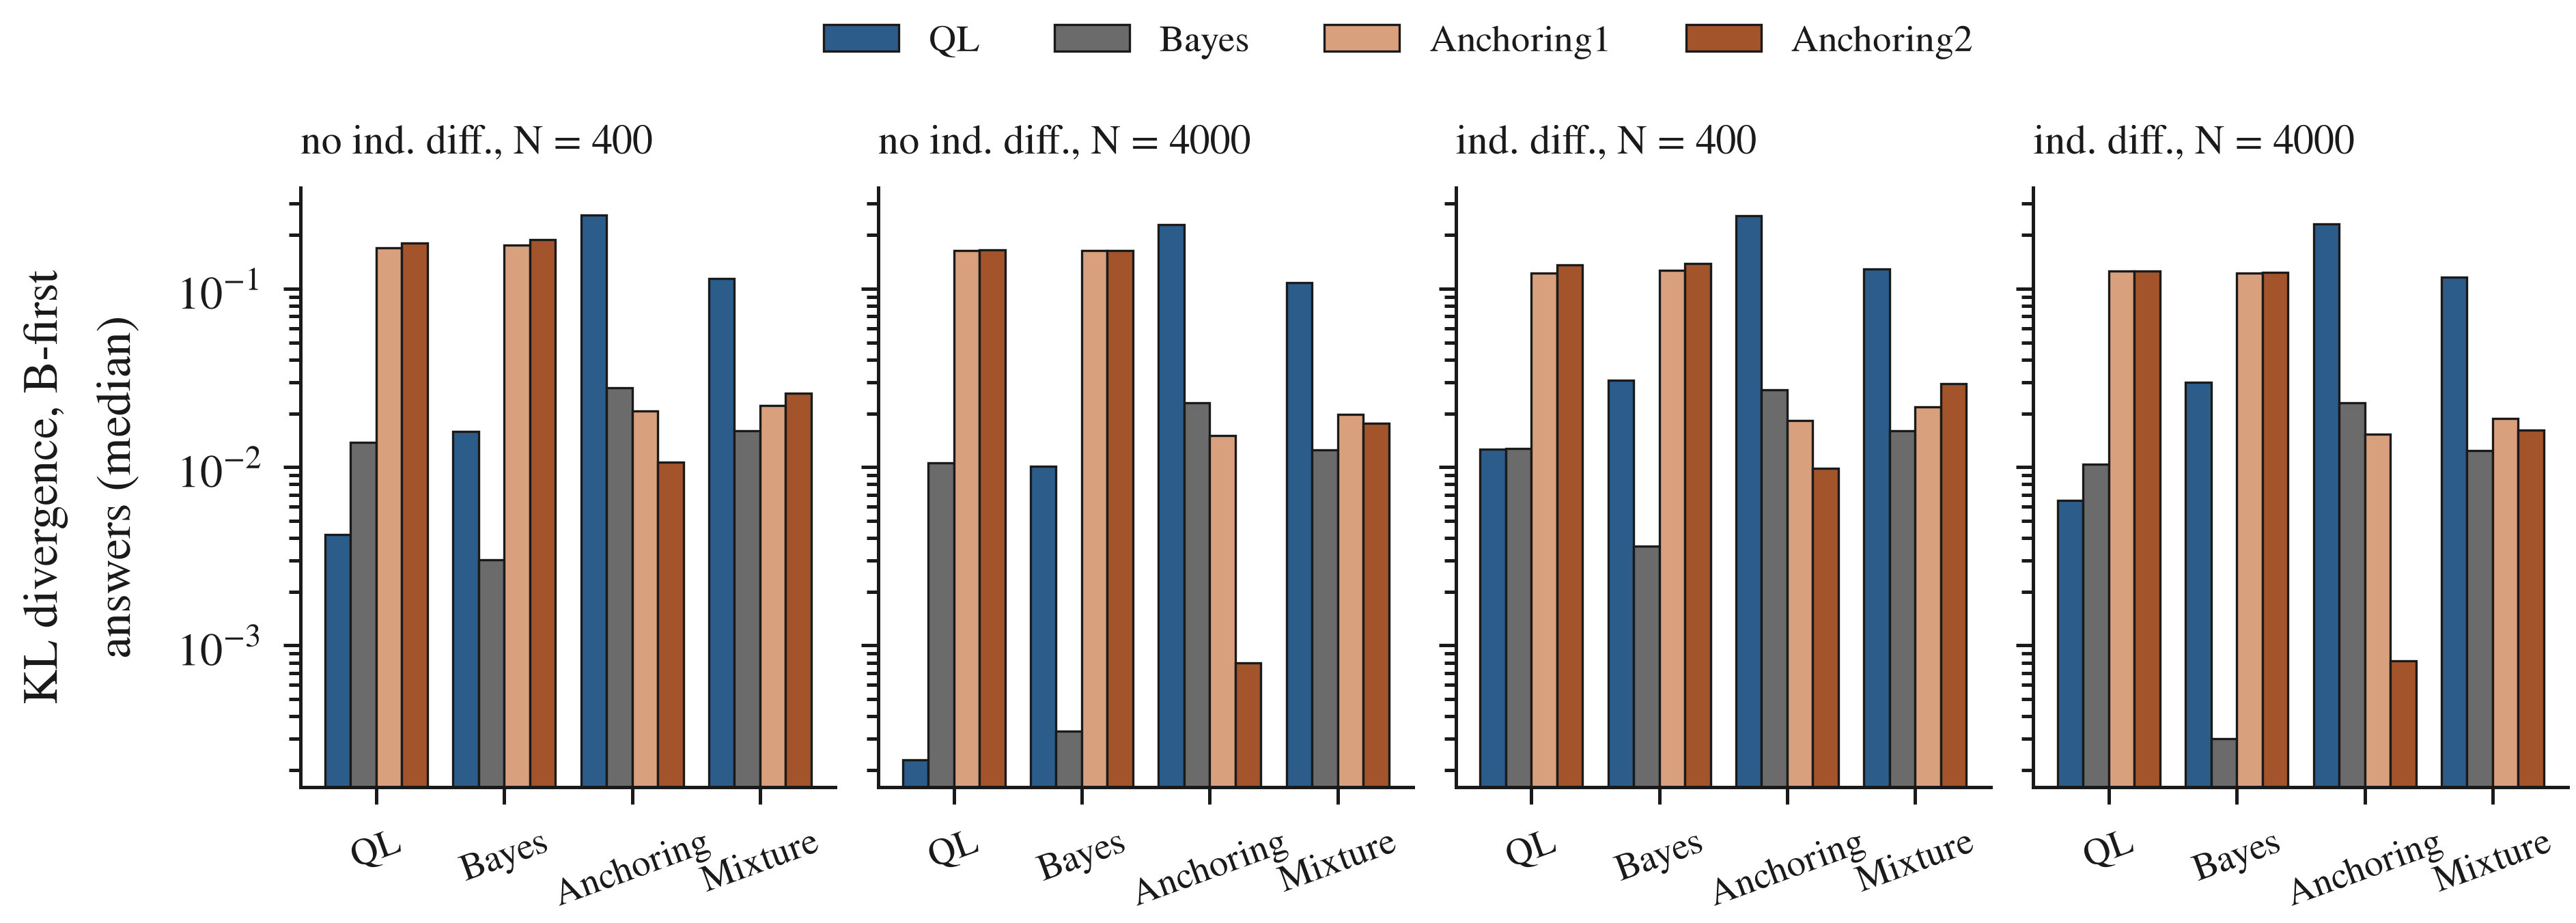
\includegraphics[width=\textwidth]{figures/Fig4_cross_order.png}
\caption{Experiment 2: Kullback--Leibler divergence between the true and the predicted B-first answer distribution (median over 30 repetitions, mean over domains, log scale), by generator, for homogeneous populations and populations with individual differences, with $N$ people answering in order AB and $N/10$ in order BA.}\label{fig:crossorder}
\end{figure*}

\subsection{Questioning Design}\label{sec:planning}
Fig. \ref{fig:planning} gives the error in the unprimed rate of the second question. The split design, which uses only first answers and no model, has an RMSE of 0.028--0.037 under every generator and population. Asking in a fixed order and reading the second answers, as a robot that ignores order effects would, gives 0.050--0.076 whenever the generator has an order effect. Model-based correction with a probe group helps only when the model is correct: with a Bayes or anchoring generator, the matching model reaches 0.021--0.030, slightly better than the split design. Under the QL generator, the QL model with a 30\% probe (0.034--0.050) does not beat the split design, because the small probe must also resolve the two-solution ambiguity of the fixed order. A wrong model is costly: the QL model applied to anchoring data gives 0.24, and the anchoring model applied to QL or Bayes data gives 0.15--0.18.

\begin{figure*}[!t]
\centering
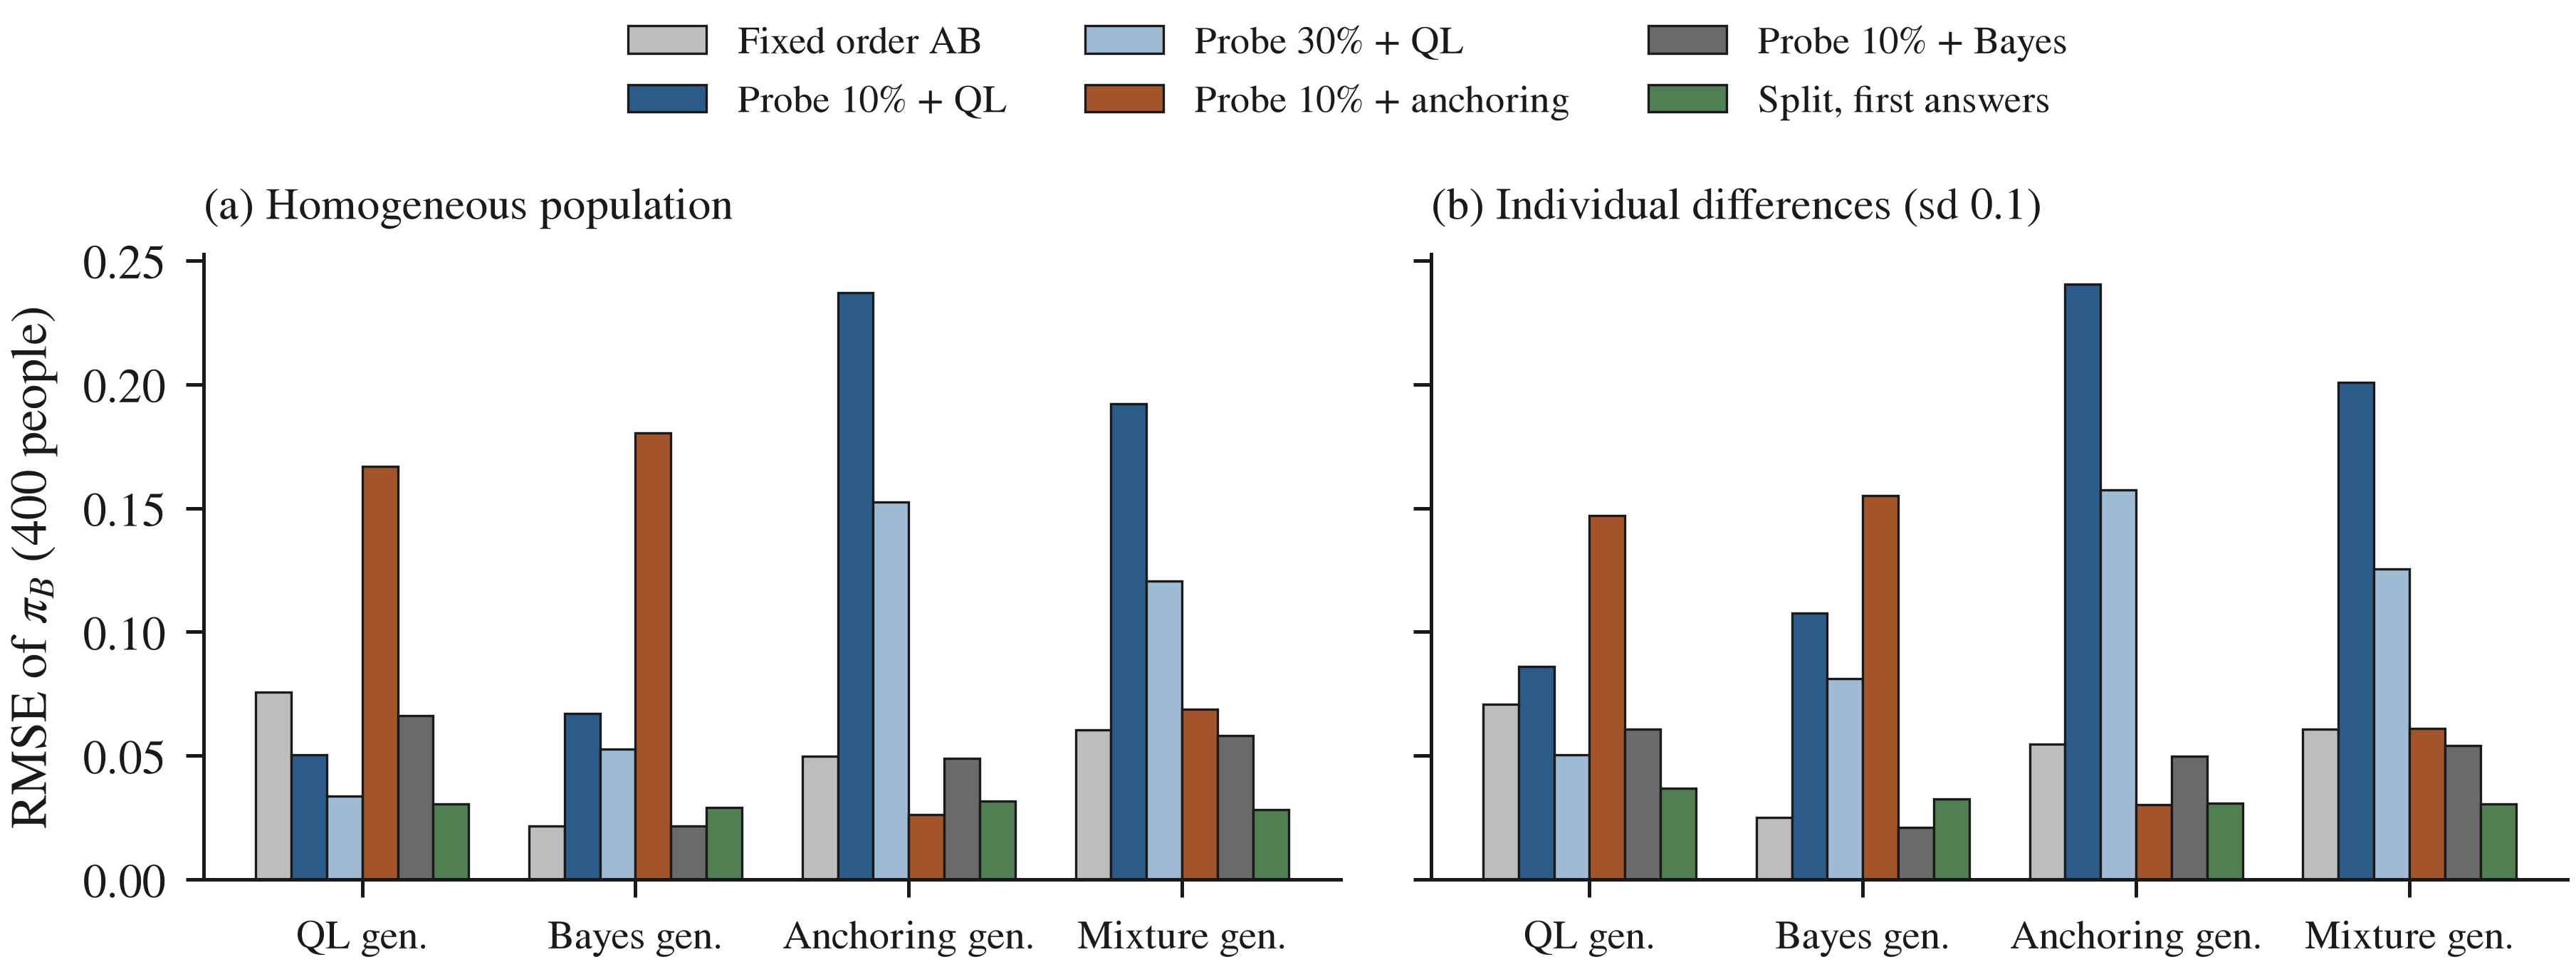
\includegraphics[width=\textwidth]{figures/Fig5_planning.png}
\caption{Experiment 3: root-mean-square error of the estimated first-position rate of question B with 400 people, by design and generator (mean over domains, 30 repetitions).}\label{fig:planning}
\end{figure*}

\subsection{Trust Dynamics}\label{sec:trust}
Under the open-system generator, the intermediate question lowers the probability of trust after the sixth hand-over from 0.725 to 0.649, a query effect of $-0.076$ (Fig. \ref{fig:trust}(a)); under the best-matching Markov model, the two conditions give the same value (0.687). BIC identifies the Markov generator in 97--100\% of data sets at all sample sizes, but identifies the open-system generator in only 3\% (100 people per condition), 27\% (400) and 93\% (1,600). A robot that always asks midway (condition C1 only) cannot learn the effect of asking: under the open-system generator, a Markov model fitted to C1 data predicts the no-question trust with a bias of $-0.06$ to $-0.08$, the size of the query effect, and the open-system model fitted to the same data is not identified (RMSE 0.15--0.17). Data from both conditions are needed.

\begin{figure*}[!t]
\centering
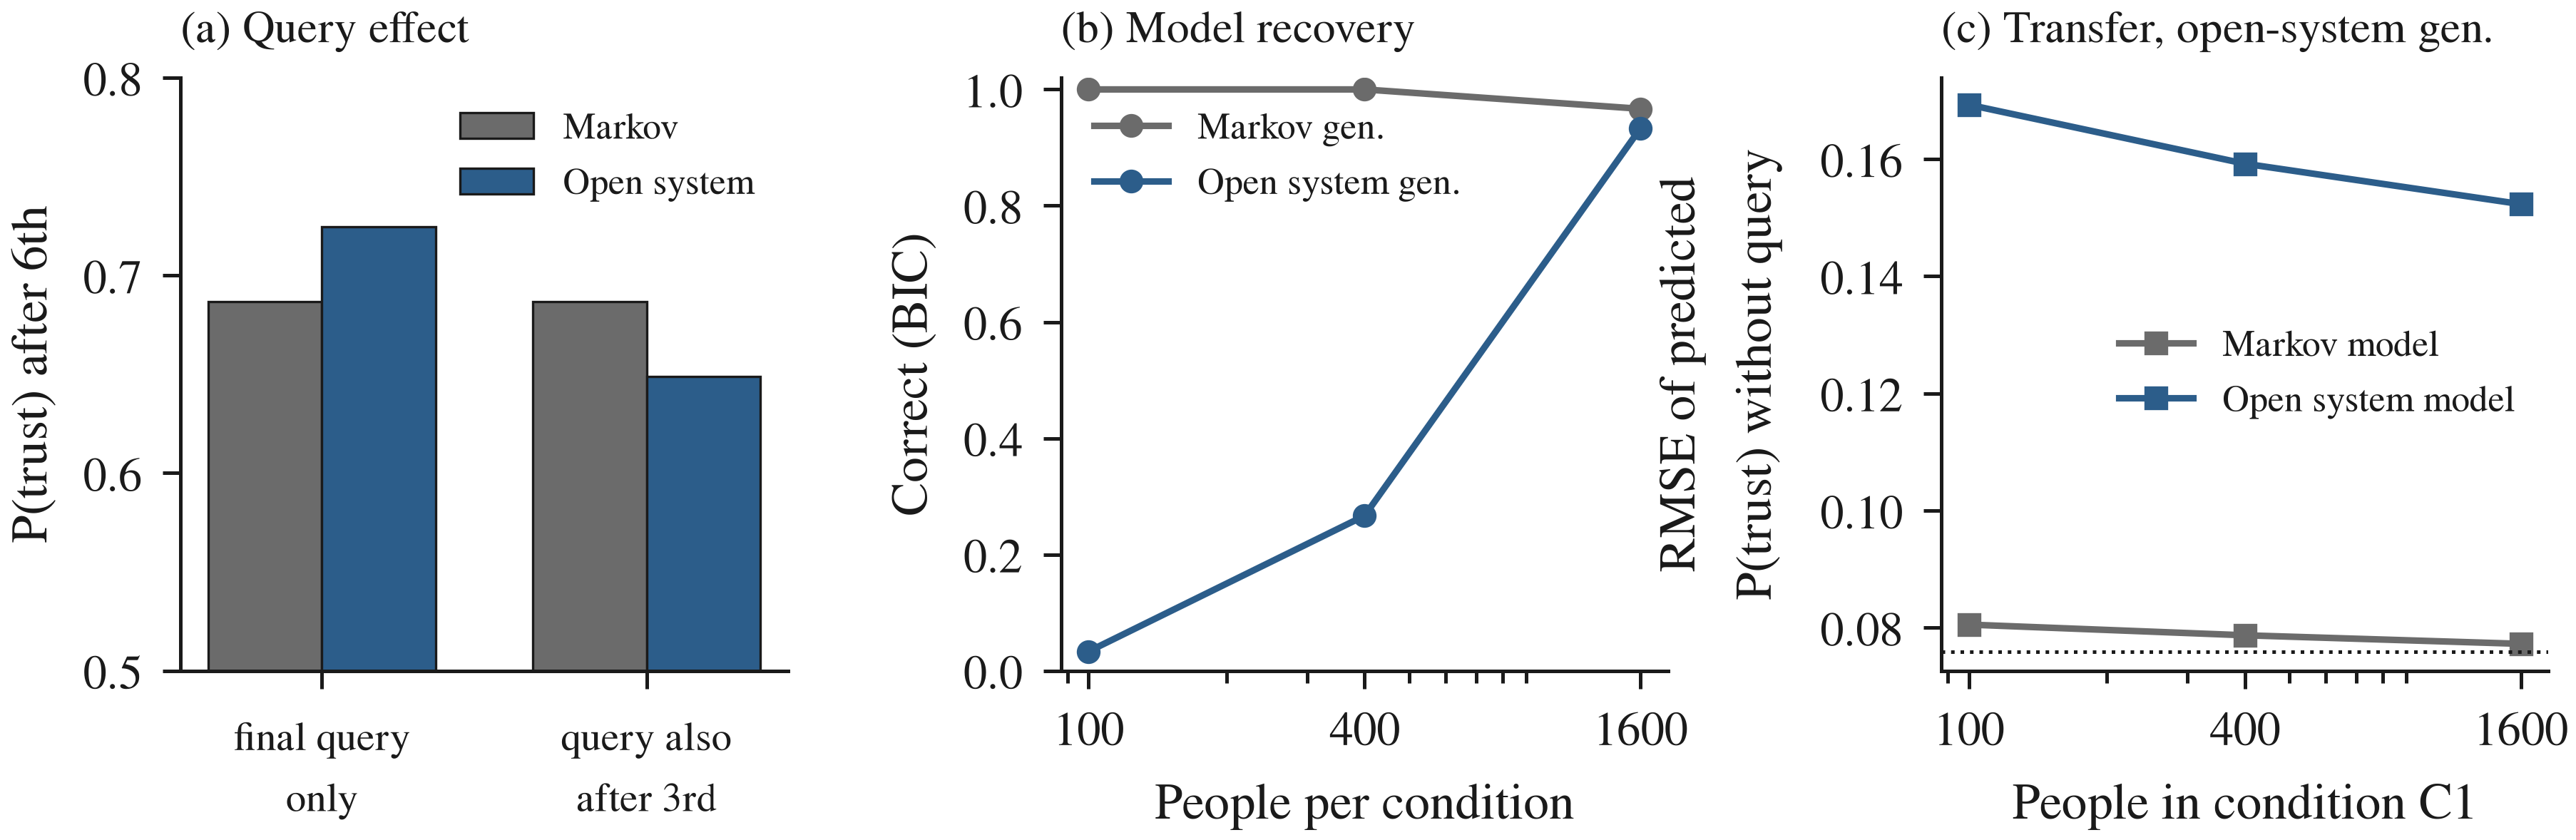
\includegraphics[width=\textwidth]{figures/Fig6_trust.png}
\caption{Experiment 4: (a) probability of trust after the sixth hand-over with and without a trust question after the third, under the open-system model and the best-matching Markov model; (b) proportion of data sets in which BIC selects the generating model; (c) error in predicting trust without the midway question from data in which it was always asked (open-system generator; dotted line, size of the query effect).}\label{fig:trust}
\end{figure*}

\subsection{Published Data}\label{sec:lit}
Table \ref{tab:lit} gives the fits to the Clinton--Gore poll. The QL model with ranks (1, 2) reproduces the four rates with a sum of squared errors of $1.4\times 10^{-5}$; the one-weight anchoring model does nearly as well ($2.5\times 10^{-5}$) and the two-weight model fits exactly, as it has as many parameters as data points. The Bayes model cannot represent an order effect ($5.7\times 10^{-3}$). The four aggregate rates therefore separate order-free from order-sensitive models but not the QL model from anchoring; the joint answer patterns, which the QQ test uses~\cite{Wang2013b,Wang2014}, are needed for that. For the Prisoner's Dilemma, the classical law of total probability requires the defection rate under uncertainty to lie between 0.84 and 0.97; the observed 0.63 lies outside. The quantum-like law reaches it with an interference phase of 1.88 rad for a belief of 0.5 that the opponent defects~\cite{Pothos2009}. One parameter is solved from one number, so this shows that the model can represent the effect, not that it predicts it.

\begin{table}[!t]
\centering
\caption{Fits to the Clinton--Gore Order Effect (Proportion Answering Yes; C Clinton, G Gore, Asked 1st or 2nd)}\label{tab:lit}
\footnotesize
\setlength{\tabcolsep}{3.5pt}
\begin{tabular}{@{}lrrrrr@{}}
\toprule
 & \textbf{C 1st} & \textbf{G 1st} & \textbf{C 2nd} & \textbf{G 2nd} & \textbf{SSE} \\ \midrule
Observed~\cite{Moore2002} & 0.50 & 0.68 & 0.57 & 0.60 & -- \\
QL (3 + ranks) & 0.498 & 0.678 & 0.572 & 0.602 & $1.4\times10^{-5}$ \\
Anchoring1 (3) & 0.498 & 0.677 & 0.573 & 0.602 & $2.5\times10^{-5}$ \\
Anchoring2 (4) & 0.500 & 0.680 & 0.570 & 0.600 & 0 \\
Bayes (3) & 0.535 & 0.640 & 0.535 & 0.640 & $5.7\times10^{-3}$ \\
\bottomrule
\end{tabular}
\end{table}

\subsection{Quantum-Circuit Execution}\label{sec:circuits}
Table \ref{tab:circ} and Fig. \ref{fig:circuits} compare circuit outputs with the analytic model. On the ideal simulators, the total variation distance is 0.003--0.007, which is shot noise at 20,000 shots, and the QQ value is within 0.004 of zero. With the noise model of the IBM FakeTorino (Heron) backend, the transpiled question circuit has depth 86--102 and 21--23 two-qubit gates; the distance rises to 0.037--0.041 in the dynamic form and 0.044--0.056 in the deferred form, and the QQ value shifts to between $-0.012$ and $-0.003$. The FakeBrisbane (Eagle) noise model gives 0.052--0.055. Depolarizing noise of 0.5\% per gate gives 0.026--0.033 and of 2\% gives 0.105--0.119, with QQ values down to $-0.039$. The trust circuit preserves the query effect under FakeTorino noise ($-0.077$ dynamic, $-0.073$ deferred, against $-0.076$ exact). No quantum hardware was used; the scripts in the repository submit the same circuits to IBM Quantum and Amazon Braket devices.

\begin{figure*}[!t]
\centering
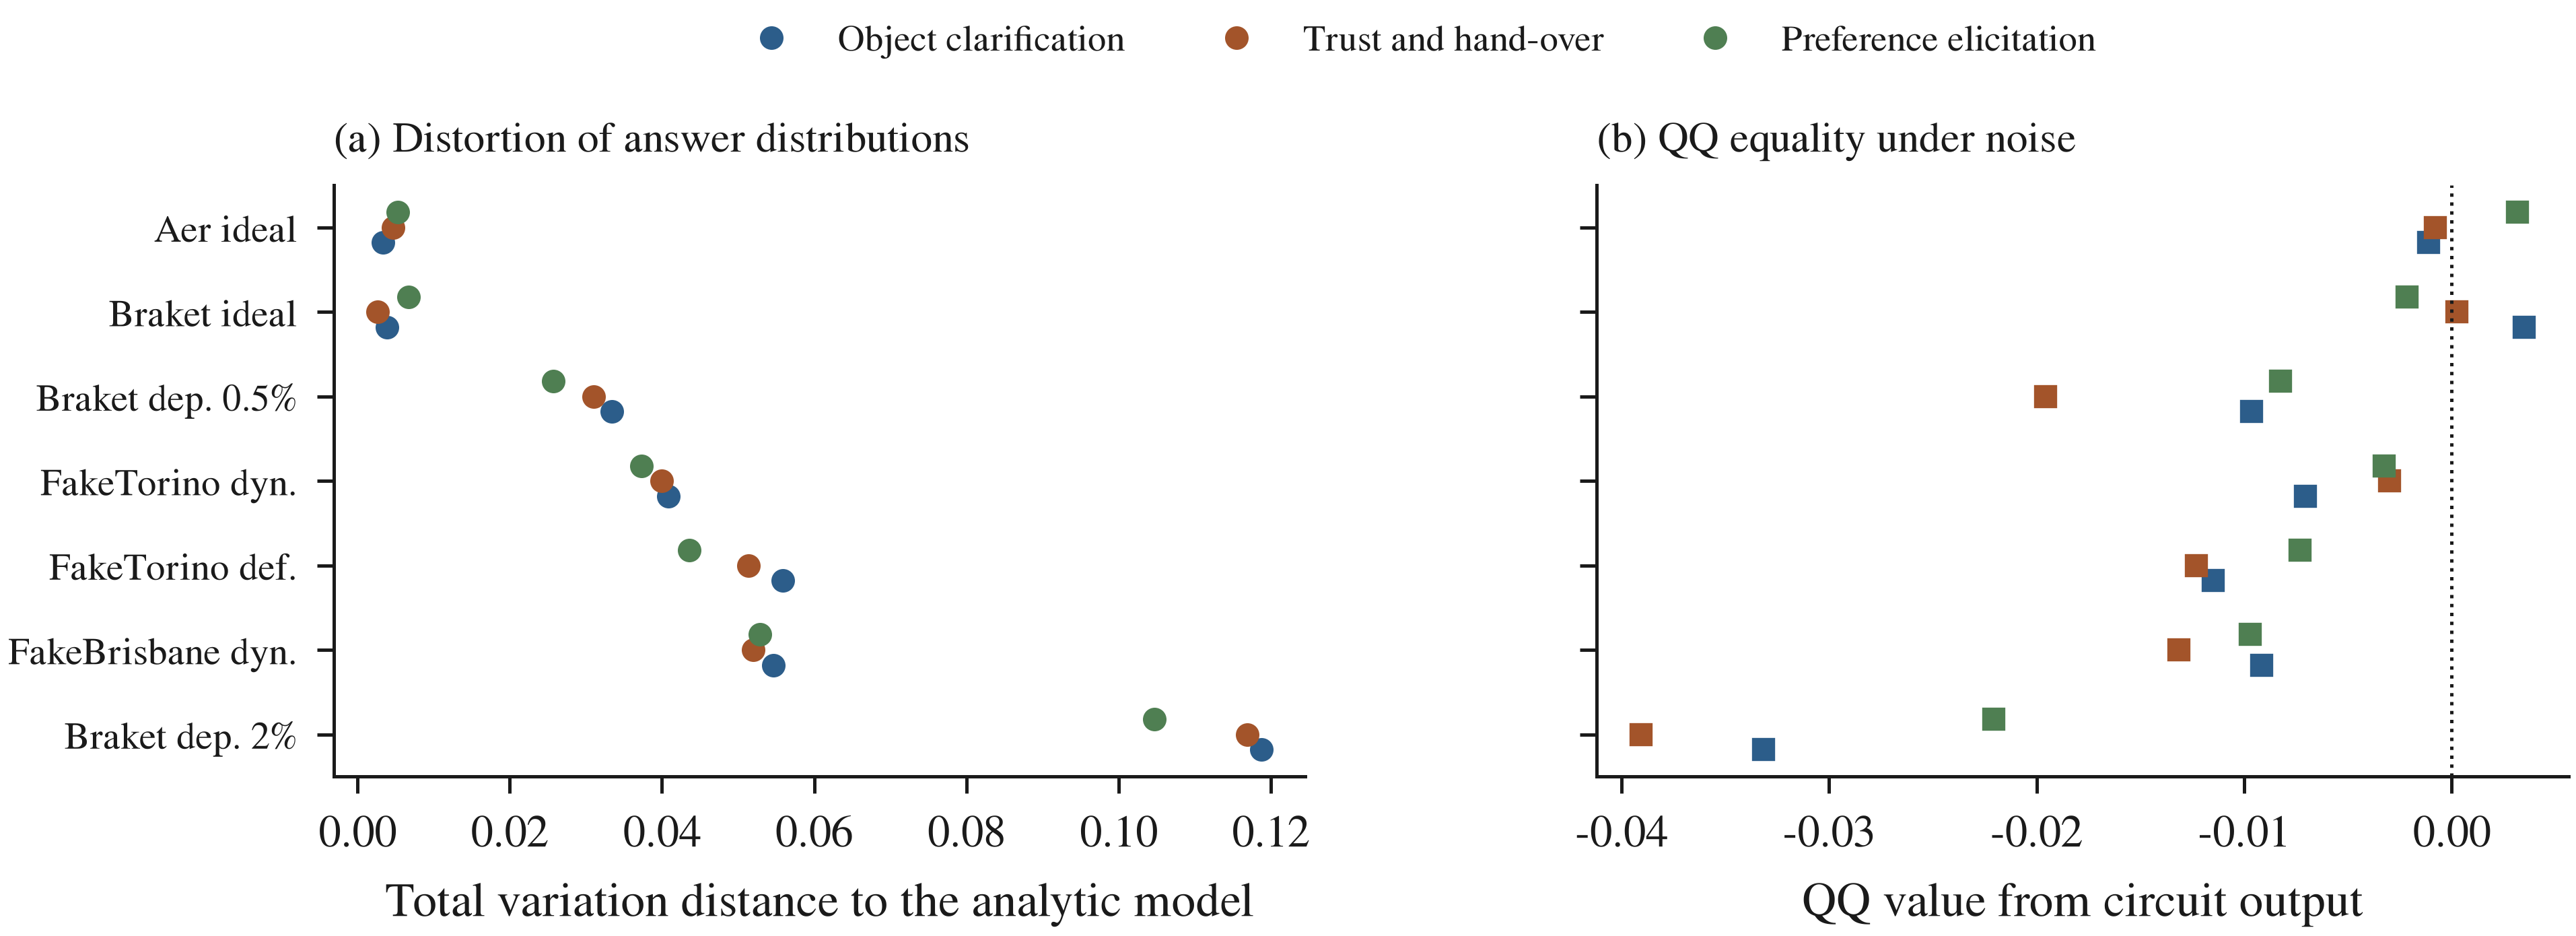
\includegraphics[width=\textwidth]{figures/Fig7_circuits.png}
\caption{Experiment 6: (a) total variation distance between the circuit output and the analytic answer distribution (mean of the two orders) and (b) QQ value of the circuit output, for each domain on ideal and noisy simulators (20,000 shots). Dyn., mid-circuit measurement; def., deferred measurement; dep., depolarizing noise per gate.}\label{fig:circuits}
\end{figure*}

\begin{table}[!t]
\centering
\caption{Question Circuits on Simulators: Range Over Three Domains (20,000 Shots)}\label{tab:circ}
\footnotesize
\begin{tabular}{@{}lll@{}}
\toprule
\textbf{Simulator} & \textbf{TVD} & \textbf{QQ value} \\ \midrule
Aer, ideal & 0.003--0.005 & $-0.001$ to 0.003 \\
Braket, ideal & 0.003--0.007 & $-0.002$ to 0.004 \\
Braket, depolarizing 0.5\% & 0.026--0.033 & $-0.020$ to $-0.008$ \\
Aer, FakeTorino, dynamic & 0.037--0.041 & $-0.007$ to $-0.003$ \\
Aer, FakeTorino, deferred & 0.044--0.056 & $-0.012$ to $-0.007$ \\
Aer, FakeBrisbane, dynamic & 0.052--0.055 & $-0.013$ to $-0.009$ \\
Braket, depolarizing 2\% & 0.105--0.119 & $-0.039$ to $-0.022$ \\
Hardware (IBM, Braket) & \multicolumn{2}{l}{\fillin{after a cloud run}} \\
\bottomrule
\end{tabular}
\end{table}


\section{Discussion}\label{sec:discussion}
\subsection{What the Quantum-Like Model Adds, and When}
The simulations give a consistent picture. The quantum-like model is the right tool when people really follow it and are similar to one another: it is then recovered reliably from a few hundred people per order and predicts the unasked order far better than the classical models. Its distinctive prediction, the QQ equality, was rejected in QL data no more often than the nominal 5\%, and it held in every circuit run to within the hardware noise. Outside these conditions the model is a liability. With small samples it reads noise as order effects; with individual differences its advantage shrinks or vanishes; and when the people follow a classical order effect, its predictions are the worst of all models. The Bayesian model, which ignores order, is never the best when order effects exist but is never far off. For a robot, this asymmetry matters more than average accuracy.

\subsection{Recommendations for Robots That Ask Questions}
Three recommendations follow. First, when the robot needs people's unprimed answers, it should randomize the order of its questions and use first answers, not correct fixed-order answers with a model; the split design was the most accurate or close to it under every generator. Second, the robot should not commit to one model of order effects. It can carry the QL, Bayes and anchoring models together, weight them by their evidence as data accumulate, and use the QQ test as a check; Experiment 1 shows that several hundred answers per order are needed before the weights become decisive. Third, asking about trust is an action, not a free reading. If trust follows open-system dynamics, a midway question lowered later trust by 0.076 in the simulation, and a robot that always asks cannot learn this effect: it must sometimes not ask. This links to help-seeking in robot planning~\cite{Ren2023,Yuan2026}, where asking is currently treated as cost-free apart from the person's time.

\subsection{Connection to Learned Orchestration}\label{sec:robot}
The companion survey frames an edge robot's controller as a meta-learned orchestrator that routes between learning modalities on calibrated confidence signals~\cite{Guru2026s3}. The human model supplies one more signal: the predictive uncertainty about the person's next answer or level of trust. The results set two conditions for using it. The signal must come from a set of models weighted by evidence, not from the QL model alone, and it must be calibrated against outcomes like the other signals, because a wrong human model is confidently wrong. The trust result adds a cost to the orchestrator's help-seeking action.

\subsection{Quantum Hardware}
The analytic models run in microseconds on a single-board computer; quantum hardware is not needed to use them. The circuits show that the representation transfers to quantum processors, and that current noise levels distort the answer distributions by about 0.04 in total variation, which is small compared with order effects of 0.07--0.08, but large compared with some QQ deviations of interest. The dynamic form is more accurate than the deferred form on the same noise model. Whether quantum hardware offers any advantage for such models, for example by evaluating many candidate human models in superposition, is an open question that this study does not address.

\subsection{Limitations}
All results except Experiment 5 come from simulated people whose parameters are illustrative, not estimated from human-robot interaction data. The models are fitted to aggregate counts, as in the survey literature; individual-level and hierarchical fitting may reduce the cost of individual differences. Only two questions are modelled, and response replicability, which standard projective models do not reproduce together with order effects~\cite{Khrennikov2014,Ozawa2021}, is not tested. The trust model has illustrative parameters and a single outcome sequence. No quantum hardware results are reported.


\section{Conclusion}\label{sec:conclusion}
This paper built and tested an order-aware model of how people answer a robot's questions and how their trust evolves when the robot asks about it. The quantum-like model reproduces published order effects as well as a classical anchoring model does and better than an order-free Bayesian model. In simulation, it can be identified and is the best predictor when people follow it and are similar to one another, but it is the worst predictor when they do not, and individual differences erode its advantage. The open-system trust model predicts that asking about trust lowers later trust, an effect that a Markov model cannot represent, that needs about 1,600 people per condition to detect, and that a robot cannot learn if it always asks. Both models run as quantum circuits and survive current hardware noise models with a total variation error of about 0.04.

The final conclusion is that quantum-like models are a useful but conditional component of a robot's model of people. They add a structure that classical models lack, and they can be tested with modest studies, but they should be used inside a set of competing models weighted by evidence, not on their own, and a robot should randomize its question order rather than correct for order effects with any single model. Whether real people interacting with real robots follow these models is the decisive open question; the pre-registered human study outlined in the repository would answer it.
